\section{Dense Rendering with a Learned Mechanics Constraint}
\label{sec:pidg-dense}
The coarse equilibrium adapter below loses image detail despite converged solves. We therefore test a distinct integration: retain PIDG's dense Gaussian appearance and temporal deformation map, and attach our frozen material decoder and inferred Gaussian interaction field as a soft training constraint. This experiment measures reconstruction compatibility, not the accuracy of a new-action forward rollout.

\paragraph{Image-connected mechanics.}
At 384 deterministic opacity-ranked support points, a 12-neighbor reference graph estimates the local deformation gradient by ridge-regularized least squares. Differentiating the shared material energy gives internal forces; central differences of the shared deformation map at fixed material support coordinates give velocity and acceleration. Sixteen spatial Gaussian kernels carry temporally interpolated vector loads and compliant targets, with positive stiffness and damping; each has 16 time knots. The nondimensional interaction is
\begin{equation}
\begin{aligned}
 f_i^{\mathrm{ext}}(t)&=g+\sum_{k=1}^{16}\omega_k(y_i)
 \big[a_k(t)+\operatorname{softplus}(s_k)(c_k(t)-y_i)-\operatorname{softplus}(d_k)v_i\big],\\
 \omega_k(y)&=\frac{\exp(-\|y-\mu_k\|^2/(2\sigma^2))}{1+\sum_j\exp(-\|y-\mu_j\|^2/(2\sigma^2))}.
\end{aligned}
\end{equation}
Here $\sigma=0.65$ in reconstruction-normalized coordinates; fixed centers $\mu_k$ are sampled from the reference support. The body-load vector $g$, temporal loads $a_k$, targets $c_k$, stiffness/damping parameters and bounded scene material descriptors are optimized jointly with dense deformation and appearance, while the learned material decoder remains frozen. A fixed acceleration scale $s_a$ from the initial reconstruction defines nondimensional units. The added loss includes $\operatorname{Huber}(\ddot y_i/s_a-f_i^{\mathrm{int}}-f_i^{\mathrm{ext}})$, with orientation, energy and parameter penalties. The support coordinates remain fixed while canonical Gaussian centers can be refined. Thus the mechanics term constrains the deformation network shared with rendering, but inference still queries the learned temporal map rather than integrating a contact solver.

\paragraph{Matched protocol.}
The three released scenes use 101/11/38 fitting/validation/test images for Balls Reaction and 135/15/50 for each of Rubber Duck and Motion Kuro. Each scene has a 50,000-step native base and four independent 5,000-step refinements from that same base: native PIDG and mechanics weights $10^{-5},10^{-4},10^{-3}$. Capacity, image order, optimizer restart and schedules are shared; refinement does not densify. Native velocity/stress networks are reinitialized in every refinement because upstream checkpoints omit them. Balls Reaction and Motion Kuro use fitting-only optical flow; Rubber Duck follows its released no-flow configuration. Supplied camera poses and released per-image depth are retained. All training uses $320\times180$ images. The largest validation foreground PSNR selects the positive-weight hybrid; checkpoint hashes are sealed before test evaluation. Balls Reaction was previously exposed in development; the other two test splits were first evaluated in this campaign. The published PIDG paper uses a different setup, so its table values are not mixed with these matched reproductions.

\begin{center}\begin{minipage}{\textwidth}
\captionof{table}{\textbf{Three PIDG scenes: matched native / dense-hybrid scores.} Each cell lists PIDG first, then our hybrid. PSNR is higher-is-better; LPIPS is lower-is-better. Larger output widths use the same 320-width trained checkpoints. Foreground PSNR guards against black-background dominance. These are 138 held images from one dataset, not 138 independent physical trials.}
\label{tab:pidg-dense}
\centering\small
\begin{tabular}{lrccc}\toprule
Scene & Width & PSNR (dB) & Foreground (dB) & LPIPS \\\midrule
Balls Reaction & 320 & 49.54 / 49.51 & 39.61 / 39.59 & 0.0004 / 0.0004 \\
Balls Reaction & 640 & 34.48 / 34.49 & 25.28 / 25.29 & 0.0086 / 0.0086 \\
Balls Reaction & 1600 & 31.64 / 31.66 & 22.41 / 22.43 & 0.0323 / 0.0323 \\
Rubber Duck & 320 & 41.82 / 41.59 & 32.60 / 32.36 & 0.0042 / 0.0044 \\
Rubber Duck & 640 & 33.20 / 33.17 & 25.50 / 25.47 & 0.0186 / 0.0189 \\
Rubber Duck & 1600 & 30.91 / 30.91 & 23.56 / 23.55 & 0.0320 / 0.0322 \\
Motion Kuro & 320 & 39.92 / 39.79 & 30.57 / 30.46 & 0.0075 / 0.0078 \\
Motion Kuro & 640 & 32.01 / 32.02 & 21.82 / 21.82 & 0.0342 / 0.0345 \\
Motion Kuro & 1600 & 29.59 / 29.60 & 19.28 / 19.29 & 0.0606 / 0.0606 \\
\bottomrule\end{tabular}\end{minipage}\end{center}

\paragraph{Outcome and checks.}
3 of three scenes meet the predeclared rendering-parity criterion at the training resolution: at most 0.5\,dB loss in both full-image and foreground PSNR and at most 0.005 LPIPS increase. This tolerance is a practical criterion, not a statistical equivalence test. All candidate validation scores and all test images are retained. The baseline repeat on Balls Reaction agrees with the earlier reproduction within 0.003\,dB. Before optimization, adding the mechanical module preserves every pixel on all 112 fitting/validation images of Balls Reaction. Energy-gradient and internal-force conservation tests pass. Ridge regularization introduces a small discrete rotation bias (maximum tested rigid-rotation energy is 0.93\% of the tested 5\% stretch energy), so exact discrete objectivity is not claimed.

\begin{center}\begin{minipage}{\textwidth}
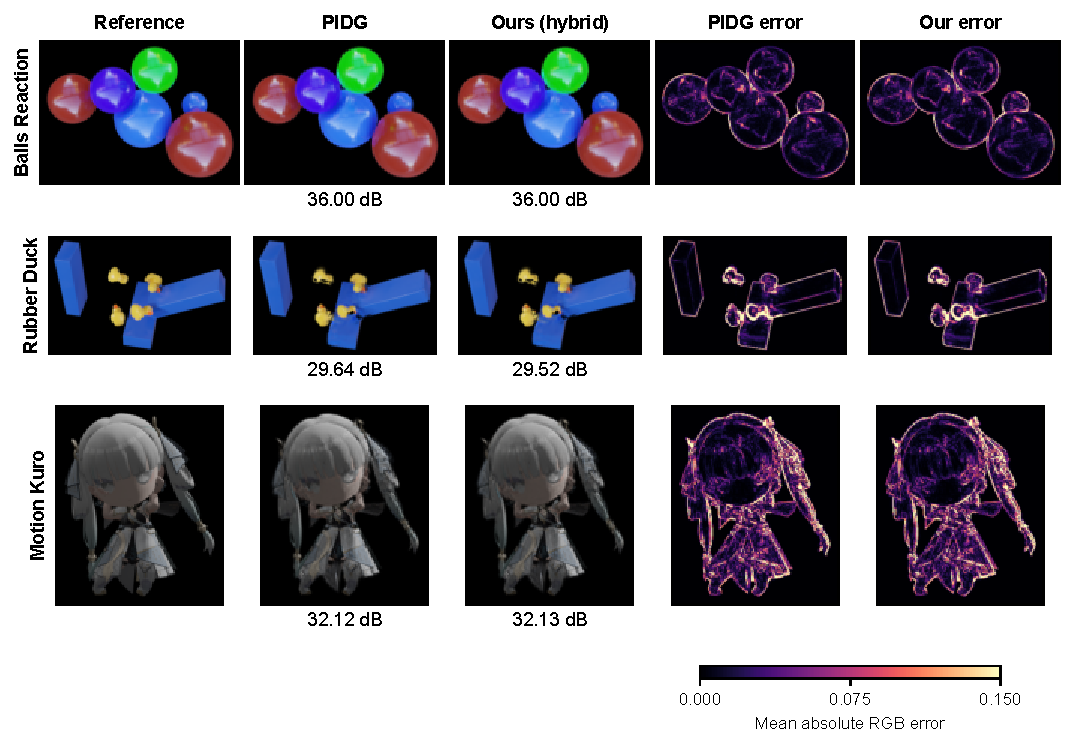
\includegraphics[width=\textwidth]{figures/pidg-dense-three-scenes.pdf}
\captionof{figure}{\textbf{Dense appearance retained across three scenes.} The middle declared test frame of each scene, rendered at width 640; identical reference-foreground crops, camera and error scale. Labels give full-frame PSNR. These examples illustrate visual agreement rather than new-action prediction.}
\end{minipage}\end{center}

\paragraph{Interpretation.}
This hybrid removes the large rendering penalty of the coarse adapter. It does not establish superior physical identification: material descriptors can approach their bounds, momentum residuals remain nonzero, and numerical neighborhood inversions are diagnostics rather than ground-truth physical errors. The scene field does not explicitly separate disconnected objects or enforce unilateral contact. Unknown mass, spatial scale and normalized frame time prevent interpreting fitted loads as calibrated SI forces. Recorded-camera reconstruction also does not quantify unobserved-camera accuracy. The following equilibrium study remains a separate diagnostic of hard mechanical coupling; its solved-state guarantees must not be transferred to this soft-constrained hybrid.
\clearpage
